\pdfminorversion=7
\documentclass[a4paper,final]{article}
\usepackage[14pt]{extsizes}
\usepackage[T1]{fontenc}
\usepackage[utf8]{inputenc}
\usepackage[english]{babel}

% --- Math ---
\usepackage{amsmath,amssymb,amsfonts}
\usepackage{nccmath}

% --- Page geometry ---
\usepackage[left=20mm, top=20mm, right=20mm, bottom=20mm, footskip=10mm]{geometry}

% --- Text/layout helpers ---
\usepackage{ragged2e}
\usepackage{setspace}
\usepackage{indentfirst}

% --- Graphics ---
\usepackage{graphicx}
\DeclareGraphicsExtensions{.jpg,.png,.pdf}
\usepackage{float}
\usepackage{wrapfig}
\usepackage{tikz}
\usepackage{pgfplots}
\pgfplotsset{compat=1.18}

% --- Captions ---
\usepackage[font=small,singlelinecheck=false,justification=centering,labelsep=period]{caption}
\renewcommand{\figurename}{Fig.}

% --- Lists ---
\usepackage{enumitem}

% --- Hyperlinks ---
\usepackage{hyperref}
\hypersetup{colorlinks=true, linkcolor=blue, urlcolor=blue}

% --- Code listings ---
\usepackage{xcolor}
\usepackage{listings}

\definecolor{codegreen}{rgb}{0,0.6,0}
\definecolor{codegray}{rgb}{0.5,0.5,0.5}
\definecolor{codepurple}{rgb}{0.58,0,0.82}
\definecolor{backcolour}{rgb}{0.95,0.95,0.92}

% --- CLIPS language definition for listings ---
\lstdefinelanguage{CLIPS}{
	keywords={deffunction, defrule, assert, retract, printout,
	          read, bind, while, do, halt, declare, not, or, and,
	          if, then, else, member\$, lowcase, lexemep, eq, salience},
	morestring=[b]",
	morecomment=[l]{;},
	sensitive=false
}

\lstdefinestyle{mystyle}{
	backgroundcolor=\color{backcolour},
	commentstyle=\color{codegreen},
	keywordstyle=\color{magenta},
	numberstyle=\tiny\color{codegray},
	stringstyle=\color{codepurple},
	basicstyle=\ttfamily\footnotesize,
	breaklines=true,
	breakatwhitespace=false,
	captionpos=b,
	keepspaces=true,
	numbers=left,
	numbersep=5pt,
	showspaces=false,
	showstringspaces=false,
	showtabs=false,
	tabsize=4,
	columns=fullflexible,
	extendedchars=true,
	inputencoding=utf8,
	literate=
	{•}{{-}}1
	{--}{{--}}2
	{---}{{---}}3
}

\lstset{style=mystyle}
\renewcommand{\lstlistingname}{Listing}
\sloppy

% --- Other document tweaks ---
\renewcommand{\arraystretch}{1.4}
\parindent=24pt
\parskip=0pt
\tolerance=2000
\flushbottom

\begin{document}
	\begin{center}
		\normalsize\bf{{MINISTRY OF SCIENCE AND HIGHER EDUCATION
		OF THE RUSSIAN FEDERATION}

			\hfill \break
			Federal State Autonomous Educational Institution of Higher Education\\
			``Peter the Great St.~Petersburg Polytechnic University''\\[10pt]}
		\hfill \break
		\normalsize{Institute of Computer Science and Cybersecurity}\\[10pt]

		\normalsize{Higher School of Technology and Artificial Intelligence}\\[10pt]

		\normalsize{Programme: 02.03.01 Mathematics and Computer Science}\\
		\vspace{50pt}

		\vspace{1pt}
		\begin{center}
Course Work Report\\
on the subject ``Graph Theory''\\
Implementation of an Expert System:\\
``Choosing a Pet Based on Given Characteristics''
		\end{center}

		\hfill \break
		\hfill \break
	\end{center}
	\small{ \bf
		\begin{tabular}{lrrl}
			\!\!\!Student, & \hspace{0cm} & & \\
			\!\!\!group 5130201/40001 & \hspace{1.5cm} & \underline{\hspace{3cm}} & \hspace{-0.3cm}Ovi Md Shamin Yasir  \\\\
			\!\!\!Supervisor, & \hspace{1cm} & \\
			\!\!\! & \hspace{0.1cm} & \underline{\hspace{3cm}} & Vostrov Aleksey Vladimirovich\\\\
			&&\hspace{3.5cm}
		\end{tabular}
		\begin{flushright}
			<<\underline{\hspace{1cm}}>>\underline{\hspace{2.5cm}} 2026
		\end{flushright}
	}

	\hfill \break
	\hfill \break
	\begin{center} \small\bf{Saint Petersburg, 2026} \end{center}
	\thispagestyle{empty}
	% END OF TITLE PAGE

\newpage
\tableofcontents


\newpage
\section*{Introduction}
\addcontentsline{toc}{section}{Introduction}

Expert systems are knowledge-based systems that operate within specific subject domains.

An expert system encodes the knowledge of a highly qualified specialist in a particular domain and is used for consultation, decision support, and solving ill-structured problems.

The goal of this course work is to implement an expert system in the CLIPS environment based on the production model for the domain ``Choosing a pet based on given characteristics''.

Minimum binary decision tree size: 4~levels, 30~nodes.


\newpage
\section{Subject Domain}

The chosen subject domain is ``choosing a pet based on given characteristics''. This knowledge domain contains information used to match the most suitable pet to a user depending on their lifestyle, living conditions, and personal preferences.

The classification attributes are chosen so that the user can unambiguously identify the most suitable pet. Key classification criteria: importance of daily interaction, willingness to walk and train the animal, preference for active or passive pet, tolerance for nocturnal activity, interest in an aquarium or a bird.

\subsection*{Why This Topic Was Chosen}

Choosing a pet is a typical ill-structured problem: there is no single algorithm for solving it, and the result depends on many subjective factors --- lifestyle, living conditions, available time, and personal preferences. Such problems are ideally suited to the production model of an expert system, since each characteristic can be expressed unambiguously as an IF-THEN rule:

\begin{quote}
IF (daily interaction is important) AND (time available for walks)\\
AND (large animal is acceptable)\\
THEN recommend a Dog
\end{quote}

The topic is relevant: in Bangladesh the number of pet owners has more than doubled in the last three years. The pet products market amounts to approximately 2~billion taka per year, growing at over 20\% annually~\cite{dailystar}.

\subsection*{How the Animals Were Selected}

All 16~animals included in the system were selected based on their popularity and availability in Bangladesh, confirmed by reliable sources:

\begin{itemize}
	\item According to The Daily Star (Bangladesh)~\cite{dailystar}, approximately 90\% of pet owners keep cats --- the most popular pet in the country. The pet market is growing at over 20\% per year.

	\item A 2024 academic study (ResearchGate)~\cite{researchgate1} found: cats --- 56.2\% of owners, birds --- 35.5\%, dogs --- 11.1\%, rabbits --- 5\% of all pets.

	\item According to Bikroy.com~\cite{bikroy} (the largest online marketplace in Bangladesh), the following animals are actively sold: dogs, cats, rabbits, parrots, pigeons, myna birds, canaries, aquarium fish, turtles, hamsters, guinea pigs, fancy rats, cockatiels, budgerigars, lovebirds, and goldfish.

	\item According to BdFISH~\cite{bdfish}, Bangladesh has more than 70 species of ornamental and aquarium fish actively sold in pet shops in Dhaka and Rajshahi.

	\item Katabon Online (Dhaka)~\cite{katabon} confirms the availability of all 16 species in physical pet stores.
\end{itemize}

Selection criterion: widely available, accessible, and safe domestic animals in Bangladesh, suitable for keeping in an apartment or house.

\subsection*{List of Animals (Expert System Facts)}

The following is the complete list of possible outcomes of the expert system:

\begin{enumerate}
	\item Dog
	\item Rabbit
	\item Cat
	\item Guinea Pig
	\item Hamster
	\item Fancy Rat
	\item Pigeon
	\item Myna Bird
	\item Aquarium Fish
	\item Goldfish
	\item Turtle
	\item Cockatiel
	\item Parrot
	\item Canary
	\item Lovebird
	\item Budgerigar
\end{enumerate}


\newpage
\section{Mathematical Description}

\subsection{Expert System and Its Properties}

An \textbf{expert system} is a computer system that uses the knowledge of domain experts to solve complex problems and provide recommendations or predictions.

Expert systems are primarily based on heuristic search rather than the execution of a known algorithm. This is one of the main advantages of expert system technology over the traditional approach to program development, and it is what allows them to handle the tasks they are designed for.

An expert system operates in two main modes:
\begin{itemize}
	\item knowledge acquisition mode;
	\item problem-solving mode (also called consultation mode, or usage mode).
\end{itemize}

\textbf{In knowledge acquisition mode}, the expert system is operated by a domain expert assisted by a knowledge engineer. In this mode, the expert uses the knowledge acquisition component to populate the system with knowledge (data), which then allows the system to solve problems from that domain independently in problem-solving mode.

\textbf{In problem-solving mode} (also called consultation mode), the end user interacts directly with the expert system, interested in the final result and sometimes in how it was obtained. Depending on the purpose of the system, the user does not necessarily need to be a specialist in the problem domain --- they consult the expert system for a result without possessing sufficient expert knowledge.

Components of the expert system structure:

\begin{itemize}
	\item \textbf{User Interface}: provides interaction between the user and the expert system. It may be graphical, text-based, or voice-based, allowing the user to ask questions, receive answers, enter data, and interact with the system. The interface must be intuitive and user-friendly.

	\item \textbf{Knowledge Base}: knowledge consists of rules, laws, and patterns obtained through professional activity in a subject domain. The knowledge base is a database containing inference rules and information about human experience and expertise. In other words, it is a set of patterns that establish links between input and output information.

	\item \textbf{Data}: data is a collection of facts and ideas in a formalised form. Data forms the basis for patterns used in prediction and forecasting. Advanced intelligent systems can learn from this data, adding new knowledge to the knowledge base.

	\item \textbf{Logical Inference Mechanism (Inference Subsystem)}: performs analysis and derives new knowledge by matching source data from the database against rules from the knowledge base. The logical inference mechanism can be represented conceptually as $\langle A,\,B,\,C,\,D \rangle$:
	\begin{itemize}
		\item $A$ --- a function that selects patterns from the knowledge base and facts from the database;
		\item $B$ --- a rule-checking function that determines the set of facts to which the rules are applicable;
		\item $C$ --- a function that determines the order of rule application when multiple rules match the same facts;
		\item $D$ --- a function that executes the action.
	\end{itemize}

	\item \textbf{Inference Engine}: the software component that identifies rule antecedents (where applicable) that match current facts. To do this, the inference engine:
	\begin{itemize}
		\item selects rules whose conditions match current facts;
		\item ranks the selected rules by priority;
		\item fires the rule with the highest priority.
	\end{itemize}

	\item \textbf{Intelligent Editor}: supports the knowledge base update mode. Allows the domain expert, assisted by a knowledge engineer, to add new rules and facts to the system.
\end{itemize}


\subsection{Production Model of Knowledge Representation}

Production knowledge models are closely related to logical models, which makes it possible to organise highly effective logical inference procedures.

The traditional production knowledge model includes the following basic components:

\begin{enumerate}
	\item a set of rules (or productions) representing the knowledge base of the production system;
	\item working memory, which stores the initial facts as well as facts derived from them by the inference mechanism;
	\item the inference mechanism itself, which derives new facts from existing facts according to the available inference rules.
\end{enumerate}

\begin{itemize}
	\item The core of the production knowledge model is the production (rule):\\[4pt]
	IF $\langle$\textit{condition}$\rangle$,\; THEN $\langle$\textit{action 1}$\rangle$,\; ELSE $\langle$\textit{action 2}$\rangle$

	\item A production consists of two parts: the condition --- the antecedent, and the action --- the consequent.

	\item Conditions can be combined using the logical operators AND and OR.

	\item Antecedents and consequents are formed from attributes and values.

	\item The database of the production system stores rules whose truth has been established in advance for a given problem. A rule fires when the facts in the database match the rule's antecedent. The result of firing is stored back in the database.

	\item General form of the production model: $N = \langle A,\, U,\, C,\, I,\, R \rangle$, where $N$ is the production name, $A$ is the application domain, $U$ is the applicability condition, $C$ is the production core (the IF-THEN rule), $I$ is the post-conditions, $R$ is a comment.
\end{itemize}


\subsection{Binary Decision Tree}

The expert system is represented as a binary decision tree --- an acyclic directed graph with cause-and-effect relationships. In a decision tree, questions are decision nodes and final outcomes are leaves.

The operation of the expert system corresponds to a path through the graph. The path consists of a sequence of steps at each of which the user decides which arc to follow from the current node. All questions are binary (yes/no).

Description of the decision tree:

\begin{itemize}
	\item \textbf{Nodes}: nodes represent states or decisions in the decision tree. Each node has certain properties, which may include conditions, variables, or factors on which the decision is based.

	\item \textbf{Edges}: edges represent transitions or branches between nodes. They define the logical sequence of decision-making and the links between different states. \textbf{There are two types of edges: a dashed edge represents the answer ``no'' and a solid edge represents the answer ``yes''}.

	\item \textbf{Conditions}: conditions define the logical expressions or predicates that must be true in order to follow a given edge. They may be based on variable values or factors defined in the expert system.

	\item \textbf{Rules}: rules are part of nodes and define the decision logic in specific states. They can be expressed as condition-action pairs or logical rules that specify what actions or conclusions to draw based on given conditions.

	\item \textbf{Conclusions}: conclusions are the outcomes or decisions that can be reached at a terminal node or leaf of the decision tree. They can be specific values, classifications, or actions to be taken based on the decisions made.
\end{itemize}

Numerical characteristics of the tree: number of nodes --- 31, number of levels --- 4, number of facts (leaves) --- 16, number of rules --- 15.

The binary decision tree constructed during this course work is shown as a diagram in Fig.~\ref{fig:diagram}.

\begin{figure}[H]
	\centering
	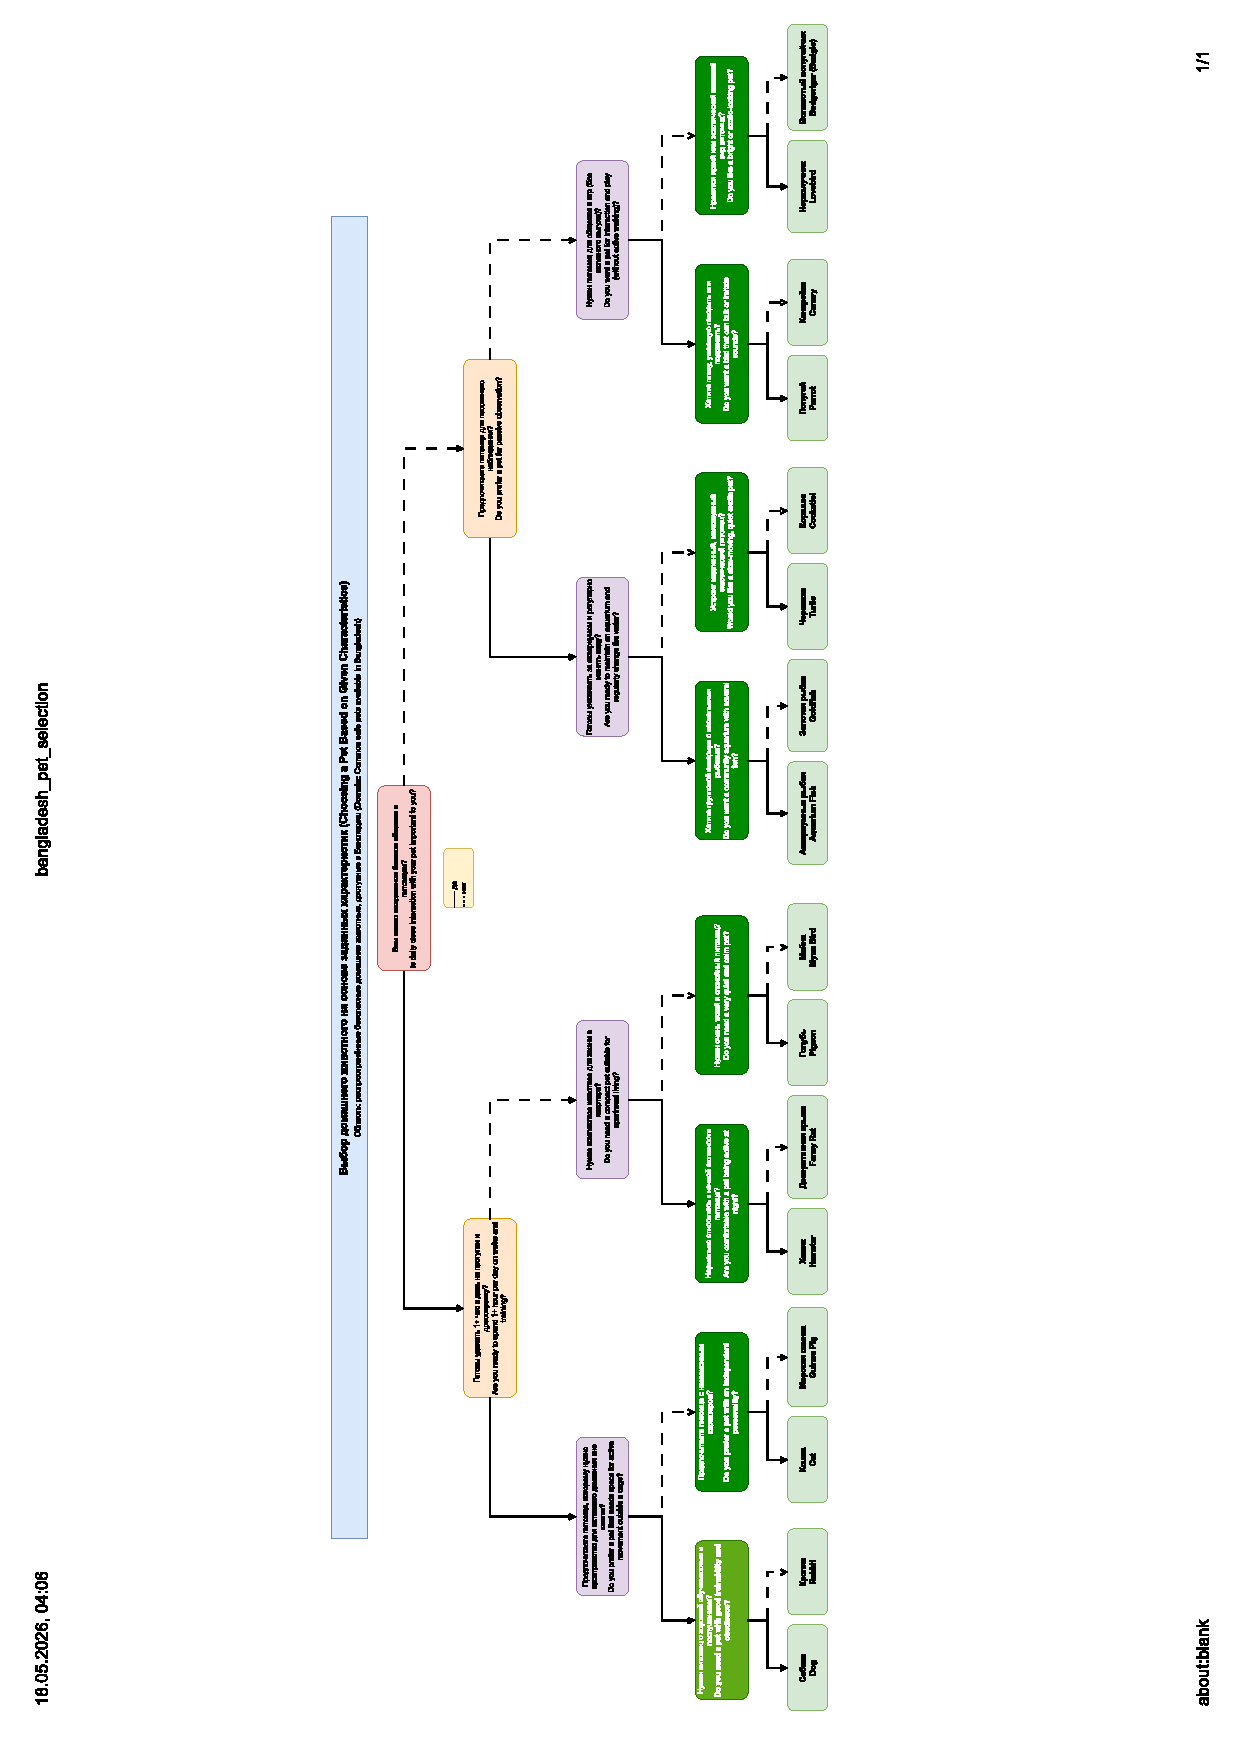
\includegraphics[width=\textwidth]{diagram.pdf}
	\caption{Binary decision tree}
	\label{fig:diagram}
\end{figure}


\clearpage
\section{Implementation Details}

The expert system is implemented in the CLIPS environment (C Language Integrated Production System) based on the production model. The knowledge base consists of 31~rules (\texttt{defrule}): 15~rules implement the decision tree nodes and 16~rules implement the leaf nodes with recommendations. CLIPS working memory stores the current facts about the user's preferences. The inference engine automatically selects and fires matching rules. This section describes the key functions and rules of the program~\cite{telematika,habаров,gavrilova}.

\subsection{General Input Function with Validation}

The \texttt{ask-question} function is a universal input function that validates user input. It accepts the question text \texttt{?question} and a list of allowed values \texttt{\$?allowed-values}. The function prints the question, reads the answer using \texttt{read}, and converts it to lowercase using \texttt{lowcase}. If the answer is not in the list of allowed values (\texttt{member\$}), an error message is displayed and the question is repeated in a \texttt{while} loop. Returns the accepted answer. The code is shown in Listing~\ref{lst:askquestion}.

\begin{lstlisting}[language=CLIPS,
	caption={The ask-question function},
	label=lst:askquestion]
(deffunction ask-question (?question $?allowed-values)
    (printout t ?question)
    (bind ?answer (read))
    (if (lexemep ?answer)
        then (bind ?answer (lowcase ?answer)))
    (while (not (member$ ?answer ?allowed-values)) do
        (printout t "  Invalid input. Please enter: " ?allowed-values crlf)
        (printout t ?question)
        (bind ?answer (read))
        (if (lexemep ?answer)
            then (bind ?answer (lowcase ?answer))))
    ?answer)
\end{lstlisting}

\subsection{Yes/No Wrapper Function}

The \texttt{yesno} function is a wrapper around \texttt{ask-question}. It accepts only the question text and calls \texttt{ask-question} with a fixed list of allowed values (\texttt{yes no y n}). It normalises the answer: if the user entered \texttt{y} or \texttt{yes}, the symbol \texttt{yes} is returned; otherwise \texttt{no} is returned. This ensures consistency: all subsequent rules in the system work only with the symbols \texttt{yes} and \texttt{no}, regardless of what the user actually typed. The code is shown in Listing~\ref{lst:yesno}.

\begin{lstlisting}[language=CLIPS,
	caption={The yesno function},
	label=lst:yesno]
(deffunction yesno (?question)
    (bind ?response (ask-question ?question yes no y n))
    (if (or (eq ?response yes) (eq ?response y))
        then yes
        else no))
\end{lstlisting}

\subsection{Recommendation Print Rule}

The \texttt{print-rec} rule has the highest priority (\texttt{salience~1000}), which guarantees that it fires before any other rule as soon as a \texttt{(rec~...)} fact appears in working memory. The rule prints the final recommendation, retracts the \texttt{(rec~...)} fact from working memory, and asserts the \texttt{(restart)} fact, thereby triggering the restart rule. The code is shown in Listing~\ref{lst:printrec}.

\begin{lstlisting}[language=CLIPS,
	caption={The print-rec rule},
	label=lst:printrec]
(defrule print-rec
    (declare (salience 1000))
    ?rec <- (rec ?item)
    =>
    (printout t crlf "Recommended pet: " ?item crlf crlf)
    (retract ?rec)
    (assert (restart)))
\end{lstlisting}

\subsection{Restart Rule}

The \texttt{restart-system} rule fires when the \texttt{(restart)} fact appears in working memory. It retracts the \texttt{(restart)} fact and asks the user whether they want a new recommendation, using \texttt{ask-question} with input validation. If the answer is positive (\texttt{yes} or \texttt{y}), the program title is printed and a new fact containing the answer to the first question is asserted in working memory, starting a new session. If the answer is negative, the message \texttt{Goodbye!} is displayed and the inference engine is stopped with \texttt{halt}. The code is shown in Listing~\ref{lst:restart}.

\begin{lstlisting}[language=CLIPS,
	caption={The restart-system rule},
	label=lst:restart]
(defrule restart-system
    ?r <- (restart)
    =>
    (retract ?r)
    (bind ?a (ask-question "Would you like a new recommendation? (yes/no): "
                            yes no y n))
    (if (or (eq ?a yes) (eq ?a y))
        then
            (printout t crlf
                "=== Expert System: Pet Selection (Bangladesh) ===" crlf crlf)
            (assert (interaction
                (yesno "Is daily close interaction with your pet important to you? (yes/no): ")))
        else
            (printout t crlf "Goodbye!" crlf)
            (halt)))
\end{lstlisting}

\subsection{Decision Tree Rules}

Each tree node is implemented as a pair of rules --- one for the ``yes'' answer and one for the ``no'' answer. Each rule: binds the matching fact to the variable \texttt{?f}, retracts it from working memory (\texttt{retract}), asks the next question via \texttt{yesno}, and asserts a new fact (\texttt{assert}). Retracting the fact immediately after the rule fires ensures that working memory is clean at the end of each session, which guarantees correct behaviour on restart. The entry rule \texttt{first} fires only when working memory is completely empty and prints the program title. Listing~\ref{lst:rules} shows a fragment demonstrating the entry rule and the first two levels of the tree; the full implementation is given in Appendix~A1.

\begin{lstlisting}[language=CLIPS,
	caption={Fragment of decision tree rules (entry rule and first two levels)},
	label=lst:rules]
; Entry point -- fires only when working memory is empty
(defrule first ""
    (not (interaction ?))
    (not (rec ?))
    (not (restart))
    =>
    (printout t "=== Expert System: Pet Selection (Bangladesh) ===" crlf crlf)
    (assert (interaction
        (yesno "Is daily close interaction with your pet important to you? (yes/no): "))))

; Level 2 -- n2 (yes branch)
(defrule interaction-yes ""
    ?f <- (interaction yes) (not (rec ?)) =>
    (retract ?f)
    (assert (walks
        (yesno "Are you ready to spend 1+ hour per day on walks and training? (yes/no): "))))

; Level 2 -- n3 (no branch)
(defrule interaction-no ""
    ?f <- (interaction no) (not (rec ?)) =>
    (retract ?f)
    (assert (passive
        (yesno "Do you prefer a pet for passive observation? (yes/no): "))))
\end{lstlisting}

\subsection{Leaf Rules (Recommendations)}

The 16~leaf rules implement the leaf nodes of the decision tree. Each rule checks for the presence of a level-4 fact and the absence of a \texttt{(rec~...)} fact. When fired, it retracts its own fact and asserts \texttt{(rec "Animal Name")}. This immediately activates the \texttt{print-rec} rule with priority 1000. The code is shown in Listing~\ref{lst:leaves}.

\begin{lstlisting}[language=CLIPS,
	caption={Leaf rules (fragment)},
	label=lst:leaves]
(defrule trainable-yes  "" ?f <- (trainable yes)  (not (rec ?)) =>
    (retract ?f) (assert (rec "Dog")))
(defrule trainable-no   "" ?f <- (trainable no)   (not (rec ?)) =>
    (retract ?f) (assert (rec "Rabbit")))

(defrule independent-yes "" ?f <- (independent yes) (not (rec ?)) =>
    (retract ?f) (assert (rec "Cat")))
(defrule independent-no  "" ?f <- (independent no)  (not (rec ?)) =>
    (retract ?f) (assert (rec "Guinea Pig")))

; ... (remaining 12 leaf rules follow the same pattern)

(defrule bright-yes "" ?f <- (bright yes) (not (rec ?)) =>
    (retract ?f) (assert (rec "Lovebird")))
(defrule bright-no  "" ?f <- (bright no)  (not (rec ?)) =>
    (retract ?f) (assert (rec "Budgerigar")))
\end{lstlisting}


\clearpage
\section{Program Results}

The result of the work is a complete program implemented in the CLIPS environment. It is launched using the commands \texttt{(load "pet\_expert.clp")}, \texttt{(reset)}, \texttt{(run)} in the CLIPS interpreter. After launch the title is displayed and the first question (the root of the binary decision tree) is asked. The user answers \texttt{yes} (or \texttt{y}) for ``yes'' and \texttt{no} (or \texttt{n}) for ``no''. The program validates input: if an invalid value is entered, an error message is shown and the question is repeated. After passing through four levels of the tree, the system displays a recommendation and offers to start a new session. Examples of program execution are shown below.

Fig.~\ref{fig:run1} shows the first program session. The user answers \texttt{y} to all four questions (path yes-yes-yes-yes): the system recommends \textit{Dog}. After the recommendation the program offers a new session and also demonstrates input validation at the restart prompt.

\begin{figure}[H]
	\centering
	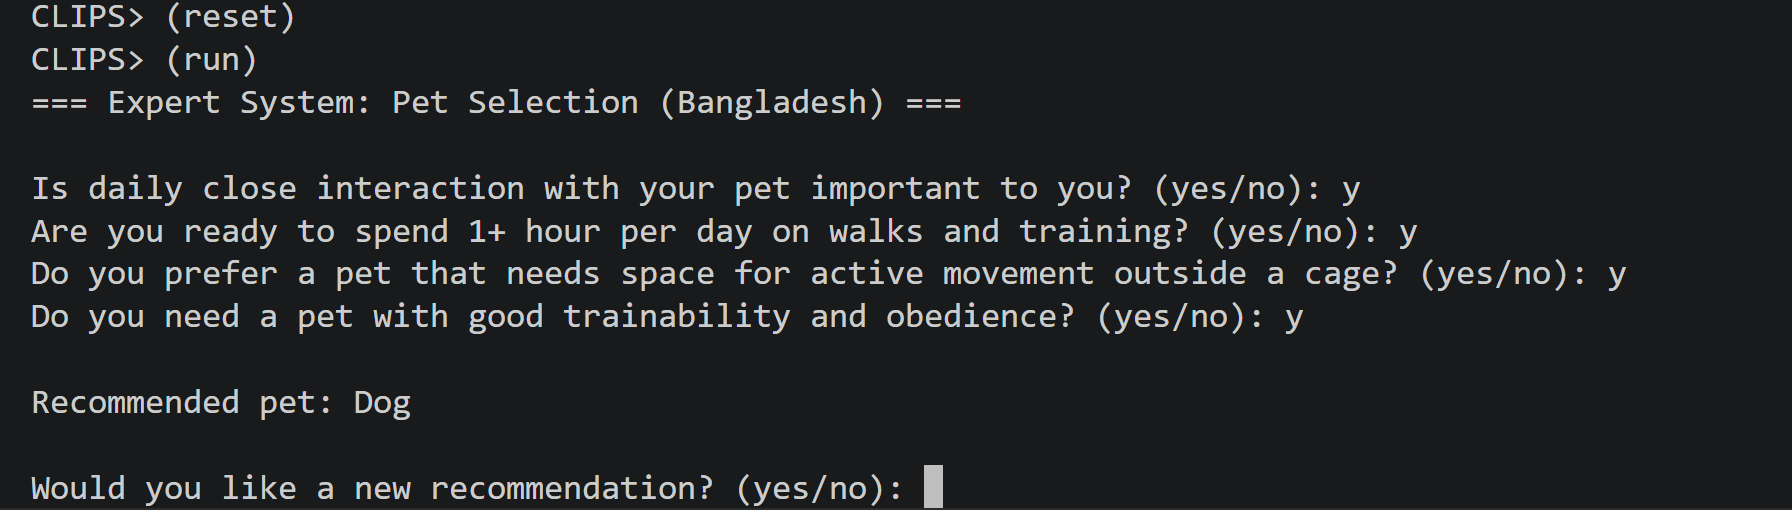
\includegraphics[width=\textwidth]{clips1.png}
	\caption{Example 1: path yes-yes-yes-yes, recommendation --- Dog}
	\label{fig:run1}
\end{figure}

Fig.~\ref{fig:run2} shows a second session with different answers. The program demonstrates correct restart behaviour: working memory is fully cleared between sessions and the system asks all questions again from the root of the tree.

\begin{figure}[H]
	\centering
	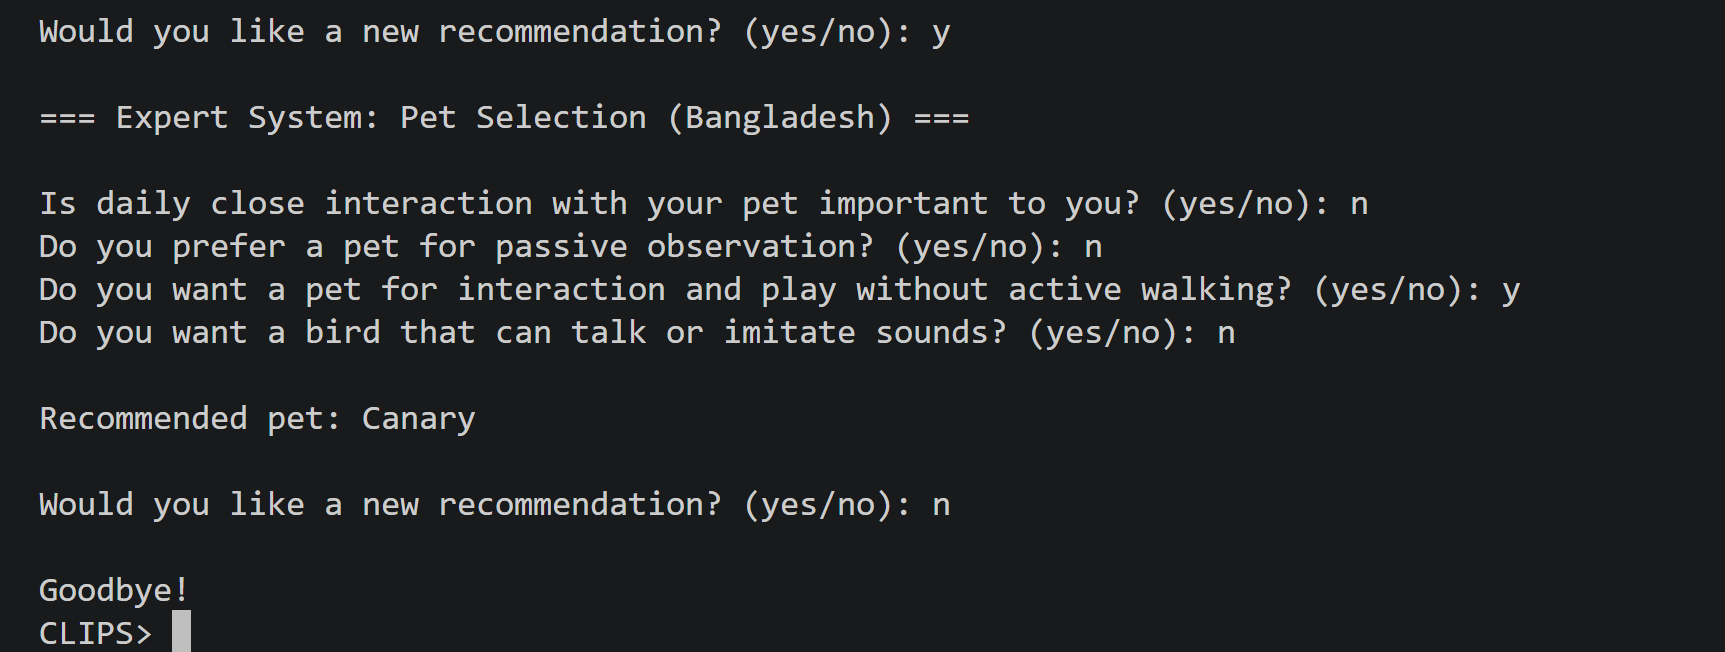
\includegraphics[width=\textwidth]{clips2.png}
	\caption{Example 2: second session with new answers and program exit}
	\label{fig:run2}
\end{figure}


\clearpage
\section*{Conclusion}
\addcontentsline{toc}{section}{Conclusion}

As a result of this course work, an expert system was implemented in the CLIPS environment on the topic ``Choosing a pet based on given characteristics (Bangladesh)''~\cite{dailystar,researchgate1,researchgate2}. The system is represented as a binary decision tree with the following numerical characteristics: number of nodes --- 31, number of levels --- 4, number of facts --- 16, number of rules --- 15. The knowledge of the implemented system is represented using the production model: the knowledge base consists of 31~rules, working memory stores the current session facts, and the CLIPS inference engine automatically controls rule activation. The system allows the user to unambiguously identify the most suitable pet based on their lifestyle, living conditions, and personal preferences.

\textbf{Advantages}

Advantages of using CLIPS and the production model:
\begin{itemize}
	\item Knowledge (rules) is separated from the control mechanism (the CLIPS inference engine): adding a new node to the tree requires only adding a new pair of rules, without modifying the control logic.
	\item The binary decision tree traversal algorithm is efficient: exactly 4 questions are required to obtain a recommendation, corresponding to the number of tree levels.
	\item The priority mechanism (\texttt{salience}) ensures a predictable rule firing order: the recommendation print rule always fires first.
\end{itemize}

\textbf{Disadvantages}

\begin{itemize}
	\item Adding or removing a node requires redesigning the decision tree and adding the corresponding rules, so the system is not completely flexible.
	\item The expert system is suitable for problems with a limited number of factors and simple interactions; more complex problems require more advanced knowledge representation methods --- semantic networks and frame-based models~\cite{gavrilova}.
\end{itemize}

\textbf{Scalability}

The program can be extended by adding new questions and animals, refining the classification criteria, or expanding the binary decision tree. Another approach to scaling is to switch to more complex knowledge representation structures in CLIPS: using \texttt{deftemplate} for structured facts, or connecting an external knowledge base~\cite{habаров}.


\clearpage
\renewcommand{\refname}{References}
\addcontentsline{toc}{section}{References}
\begin{thebibliography}{99}

	\bibitem{dailystar}
	``Market for pet food, accessories growing'' / The Daily Star.~---
	URL: \url{https://www.thedailystar.net/business/economy/news/market-pet-food-accessories-growing-3422306}
	(accessed: 11.05.2026)

	\bibitem{researchgate1}
	The evolving paradigm of pet animal rearing in Bangladesh / ResearchGate.~---
	URL: \url{https://www.researchgate.net/publication/388758458}
	(accessed: 11.05.2026)

	\bibitem{researchgate2}
	Navigating Pet Welfare in Bangladesh: A Multilayered Analysis of Ownership,
	Ethics and Service Accessibility / ResearchGate.~---
	URL: \url{https://www.researchgate.net/publication/398122556}
	(accessed: 11.05.2026)

	\bibitem{bikroy}
	Animals \& Pets for sale in Bangladesh / Bikroy.com.~---
	URL: \url{https://bikroy.com/en/ads/bangladesh/pets-animals}
	(accessed: 11.05.2026)

	\bibitem{bdfish}
	Aquarium Fishes of Bangladesh: Part-1 / BdFISH Feature.~---
	URL: \url{https://en.bdfish.org/2011/01/aquarium-fish-bangladesh-1/}
	(accessed: 11.05.2026)

	\bibitem{katabon}
	Katabon Online --- Best Quality Pet Supplies (Dhaka pet market).~---
	URL: \url{https://katabononline.com/}
	(accessed: 11.05.2026)

	\bibitem{dailybizeyе}
	The Rising Trend of Pet Ownership in Bangladesh / Daily Business Eye.~---
	URL: \url{https://www.dailybusinesseye.com/todayspaper/paper/4183}
	(accessed: 11.05.2026)

	\bibitem{habаров}
	Khabarov~S.\,P. CLIPS --- a language for building expert systems.~---
	Saint Petersburg, 2013.~--- 80~p.

	\bibitem{gavrilova}
	Gavrilova~T.\,A., Chasikov~A.\,P. Development of Expert Systems. The CLIPS Environment.~---
	Saint Petersburg: BHV-Petersburg, 2003.~--- 393~p.

	\bibitem{telematika}
	Section ``Telematika'' / electronic text.~---
	URL: \url{https://tema.spbstu.ru/tgraph/}
	(accessed: 11.05.2026)

\end{thebibliography}


\clearpage
\section*{Appendix A1. File pet\_expert.clp}
\addcontentsline{toc}{subsection}{Appendix A1. File pet\_expert.clp}
\label{app:clips}
\lstinputlisting[language=CLIPS, breaklines=true]{../pet_expert.clp}

\end{document}
